\documentclass[prl,reprint,showpacs,floatfix,nofootinbib]{revtex4-1}
\usepackage{epsfig,graphics,float,amsmath,mathtools}
\usepackage[colorlinks=true,citecolor=blue]{hyperref}
\usepackage{microtype,setspace,siunitx,physics,epsfig,graphicx}
\usepackage[caption=false]{subfig}
\usepackage{xcolor}
\usepackage[export]{adjustbox}
\usepackage{nameref,physics}
\usepackage{blindtext}
\captionsetup[subfigure]{labelformat=brace}
\usepackage[english]{babel}
\usepackage[normalem]{ulem}
\useunder{\uline}{\ul}{}
\usepackage{graphics}
%\definecolor{originblue}{RGB}{139,255,167}
%\definecolor{origingreen}{HTML}{fdae61}
%\addbibresource{}

\begin{document}
\title{Machine Learning for Video Analysis in Experimental Physics using Simulated Training Data: Particle and Topological Defect Identification and Tracking}
% Alternative titles:
%Generating Simulated Data for Machine Learning Training Sets: Particle and Topological Defect Identification and Tracking
\date{\today}
\author{Eric~N.~Minor}
\author{Stian~D.~Howard}
\author{Adam~A.~S.~Green}
\author{Cheol Park}
\affiliation{Department of Physics and Soft Materials Research Center, University of Colorado, Boulder, Colorado, 80309, USA}

\begin{abstract}
    \blindtext{}
\end{abstract}

\maketitle

\section{Introduction}

The application of machine learning to physics is a field of active study. Machine learning methods have been employed to solve problems in condensed matter physics such as phase classification \cite{deng_machine_2017}\cite{carrasquilla_machine_2017}\cite{beach_machine_2018}, spin analysis\cite{wang_machine_2017}, and defect identification\cite{walters_machine_2019}. These applications have all worked off of theoretical or simulated data, leaving experimental applications of machine learning for physics research largely unexplored. 

In experiments where data is collected through video capture, it is often the case that the most difficult and time consuming step is extracting the location, sizes, and counts of relevant objects in each image. In many cases, human analysis of hundreds or thousands of individual frames is required to generate a large enough dataset for meaningful analysis to be conducted. This can be extraordinarily time intensive and inefficient to do on all but the smallest of scales. %ADD CITATIONS 

Computational methods for automatically extracting information from images often suffer from inaccuracy and lack of generality, with each tracking method being highly specialized to one application. We developed a machine learning and image augmentation pipeline using modern deep-learning approaches to facilitate the swift training of models for identifying objects in images. Hand annotating data for training is highly time consuming and prone to errors, which makes simulating data with annotations desirable when training a model. In order to make simulated data viable for training models meant for usage on real world data, it is necessary to enhance simulated data by adding noise and artifacts to emulate experimental data for the purpose of increasing model robustness. These techniques, of simulating data to train a model for use on real data, have the potential to greatly accelerate video based research by eliminating the need to manually track objects, develop different pipelines for each object, or hand annotate training data. %As long as a decently sized set of annotated images can be obtained, a model can be trained capable of automating tracking.

Our specific use case is the tracking of topological defects in smectic C films, with training being done on simulated images based on the XY model. Liquid crystal films are composed of discrete layers of molecules constrained to their individual layer while maintaining fluidic freedom within the layer. In smectic C films, molecules align with their neighbours, causing the fluid to have a consistent orientation described by the c-director. The orientation of the C-directors can be observed by using a pair of crossed polarizers. Topological defects occur in locations where the molecules are unable to align with all the surrounding molecules, causing an inconsistency in the overall C-director orientation. 

% - Intro to LC systems
%   - Basics of islands
% Regions where there is an inconsistency in the layer count are referred to as islands. Islands can be easily observed through a camera as regions of higher light intensity due to the higher reflectivity of the film in those regions. Islands will tend to move with the surrounding fluid allowing them to be used as a tracer particles for the fluid movement

%   - Basics of topological-defects -- Adam needs to help with this.

% - Island tracking - current methods are inflexible/expensive(computation/human time)/difficult
% - Lack robust tool for multiple things (different scripts/methods for islands,defects, etc.)
% - We use 'off-the-shelf' code for ML
%All of these methods are highly rigid, however. For every application (defect tracking, island tracking, different camera settings) significant modifications are needed to read the images, identify features, and new analysis pipelines outlined to process the information. We created a general purpose pipeline for running simulations, enhancing the simulated images, training a model, and using that model to annotate real data.. Additionally only off-the-shelf ML and tracking libraries were used, while all training data was simulated to eliminate the need of human annotations to train the model. However, hand annotated images were used validation can also be used for training if needed.

% - Applicability test with islands -- complex use/flexibility tested with defects
%Island tracking, a relatively simple application of Machine Learning, allows for a simple test of the %applicability of Machine Learning, trained on simulated data, on experimental data. Topological defect tracking, a %high complexity problem, allows for testing the flexibility and robustness of the methodology.
%

\section{Experimental System}

%One of the main goals of the pipeline is to generate a machine learning model capable of making useful detections on real world data. 

In order to confirm the veracity of our system, we collected physical data from a typical topological defect experiment.
To generate data for training the machine learning system, we used a simulation to generate perfectly annotated images and then ran those images through a data enhancement pipeline.

%and a simulation setup. For physical data, we used the same methods typically used for topological defect experiments. We used simulations to generate well annotated images of textures we expected to see in the experiments, and passed them through a data enhancement pipeline.

%To confirm the veracity of our ML pipeline, we collected real data from physical experiments to validate the model. A complementary simulation was constructed to model the experimental system for the purposes of generating training data for the machine learning model. 

%To perform this experiment, where we test the viability of using a ML pipeline trained with simulation data on real experimental data, we need both an experimental system and a complementary simulation of the system to generate the training data. 

\subsection{Experimental Defect Data}

At the center of our setup is a pressure chamber with an open aperture on the top to draw a film over. When pressure is provided to the chamber through a tube, the film bulges outward. A valve on the tube is then opened to the atmosphere, rapidly equalizing the pressure in the chamber, generating defects in the film. The valve is controlled by a computer program that, upon reaching a predetermined pressure difference between the chamber and atmosphere, will open the valve, trigger the high-speed camera recording, and start saving pressure readings. 

% Confirm 

Smectic C liquid crystal defects can be visualized with partially or fully crossed polarizers. In our setup, polarized light is shined perpendicularly onto the film. The reflected light is collected into a microscope where it passes through a partially crossed polarizer. A high speed camera (Phantom V12.1) records the reflected light at 500 frames per second, and an exposure time of 1900 $\mu$s in gray-scale.

\begin{figure}
  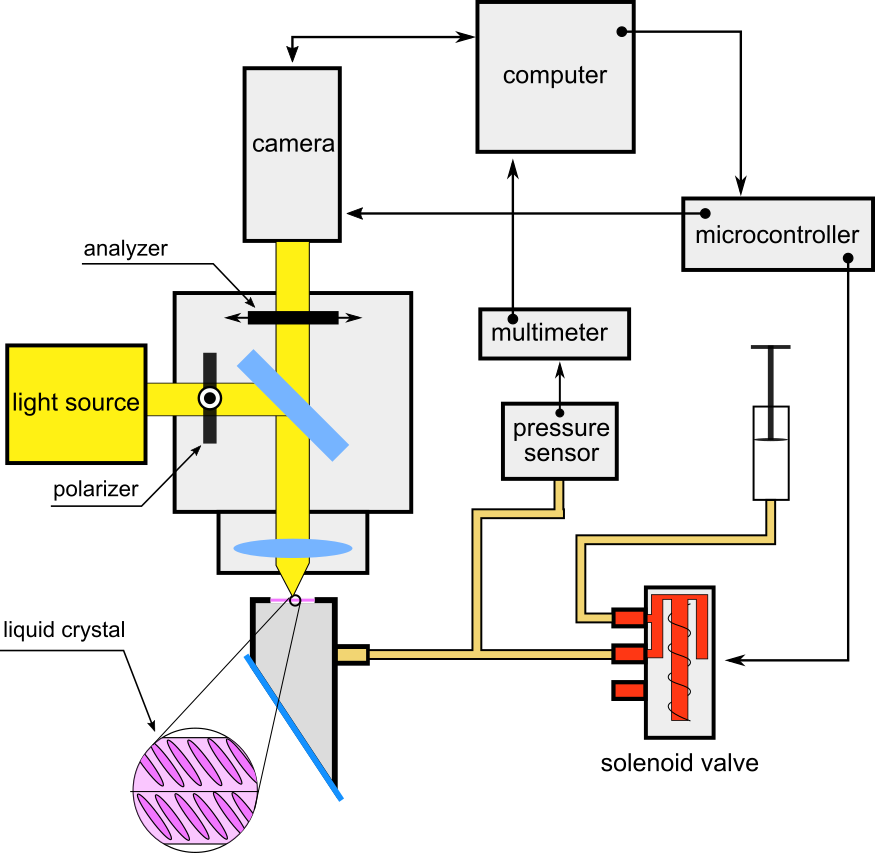
\includegraphics[width=\linewidth]{quench-schematic.png}
  \caption{Sketch of the quenching setup}
  \label{fig:Setup Sketch}
\end{figure}

Each video lasts 12.2 seconds, capturing the entirety of the short term dynamics. Images are 1104x800 and have a 12 bit pixel precision, allowing for high contrast to be gained in post processing. When the polarizers are fully crossed, the reflected light is so dim that the images turn out fully black at the exposure time used -- a value which can't be increased without significant reductions to frame rate. Partially crossed polarizers are a middle ground between a sufficient light intensity reaching the camera's CCD and giving a clear image of the relative C-director orientations.

We used PM2\cite{harth_episodes_2016} to form a film that exists in a Smectic C phase at room temperatures. The heat chamber provides additional control of film state: increased temperatures cause faster annihilation of the defects, while lower temperatures may reduce noise and island formation. In extreme circumstances, the heat chamber may prevent phase changes due to large temperature shifts in the lab environment. 

\begin{figure}
  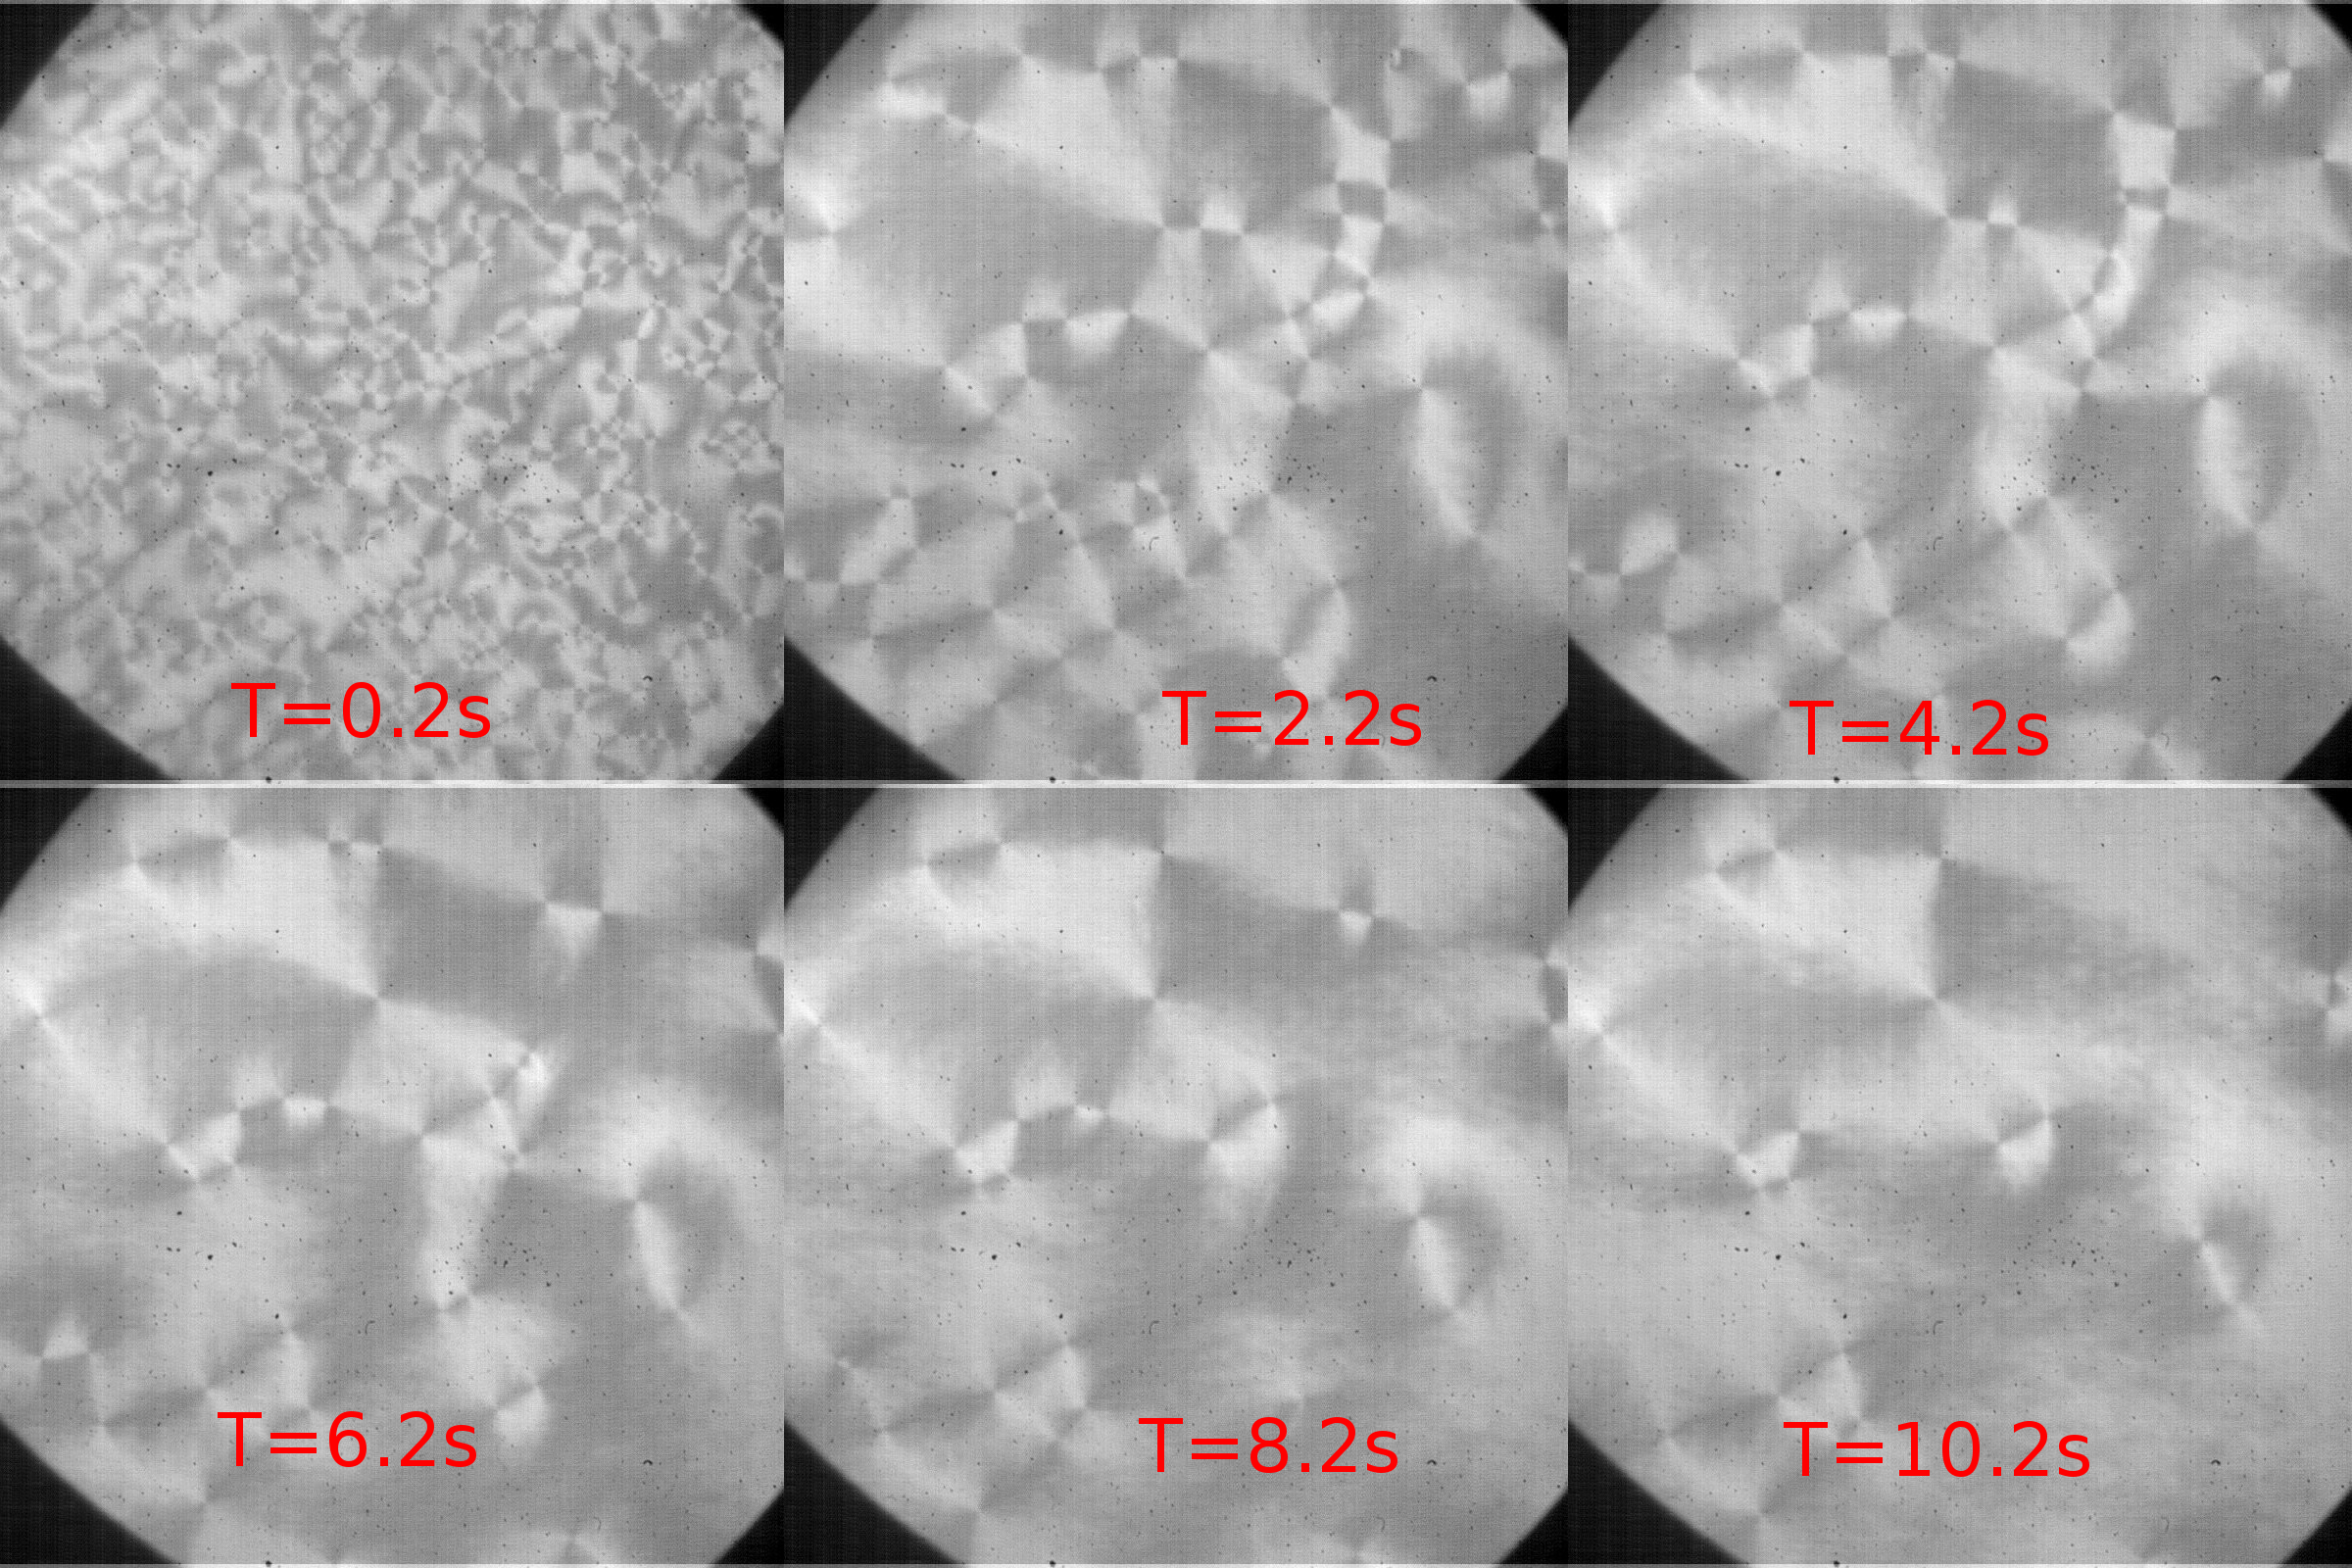
\includegraphics[width=\linewidth]{film.png}
  \caption{Time evolution of a film}
  \label{fig:frames}
\end{figure}

\subsection{Simulation Data}
%\ Need Adam to help with this section

Two methods were used to generate images for training the machine learning models to detect topological defects. The first method, which randomizes defect counts and locations, outputs a Schlieren\cite{nehring_schlieren_1972} texture with defects in the given locations. This method can output very clean, perfectly annotated images. However, it only produces an arbitrary image with the corresponding Schlieren texture rather than simulating the physics to produce the image. This simulation method will be referred to as the 'random defect' simulation.

The second method is based on a Landau-Ginzburg implementation of the XY model\cite{jelic_quench_2011} to simulate the physical behavior of defects in the film. In the initial state, the C-director of each pixel is chosen randomly. The simulation is then allowed to evolve resulting in defects forming and annihilating naturally. This method also gives thermal noise to the system, increasing the similarity of the output images to experimental images.

\begin{figure}
  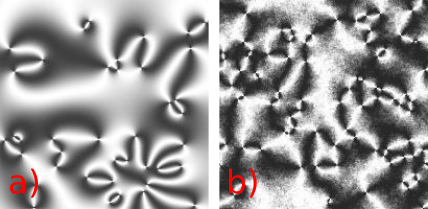
\includegraphics[width=\linewidth]{simulations.png}
  \caption{Typical image from simulation. a) uses a crossed polarizer angle of 50 degrees and randomized defect locations. b) uses an XY model where defect count decreases over time}
  \label{fig:RandomDefect}
\end{figure}

%
%\section{Island Tracking}

%Islands are frequently encountered while studying liquid crystal thin films, and are defined as the regions of the film where additional layers are present relative to the surrounding film. The extra layers provide additional reflection causing the regions to visually appear brighter -- particularly so in a black and white camera where they will appear as regions of the film with different intensities. Islands move in the film along with the surrounding fluid, allowing us to use them as markers which we can track to characterize the flow of the fluid film.

%There are two main techniques used to identify these flows using markers: particle image velocimetry (PIV) which employs Eulerian measurement techniques, and particle tracking velocimetry (PTV) which employs Lagrangian measurement techniques. At the crux of the matter, the difference is that PTV tracks a particle through time to determine flow, while PIV identifies flow by measuring marker movements at specific locations, but not worrying about where the markers came from or goes to in the future. In previous experimentation, we have used both PIV (OpenPIV) and PTV (racetrack experiment) to identify flow in liquid crystal films, with varying results. Considering they rely on a high degree of accuracy in particle characterization in images, these tools are highly rigid and specialized placing restriction on how and what data we can analyze. 

%Employing machine learning, we hope to overcome some of the limitations of these methods by simplifying the process of tracking markers in varying image qualities and conditions. A machine learning algorithm trained to identify islands of multiple sizes, intensities, shapes, and lighting conditions that would traditionally inhibit the capabilities of standard identification algorithms. 

%\subsection{Simulation Data}

%Considering the relative simplicity of visually identifying islands in an image, the simulation aspect for this is very straight forward. Images were prepped by generating a random number of islands with random size and intensity on a picture (We haven't actually trained anything yet, so we still need to figure out if we even need any additional noise). Several thousand of these images can be easily and quickly generated, with perfect training annotations of island locations and sizes.

%\begin{figure}
%  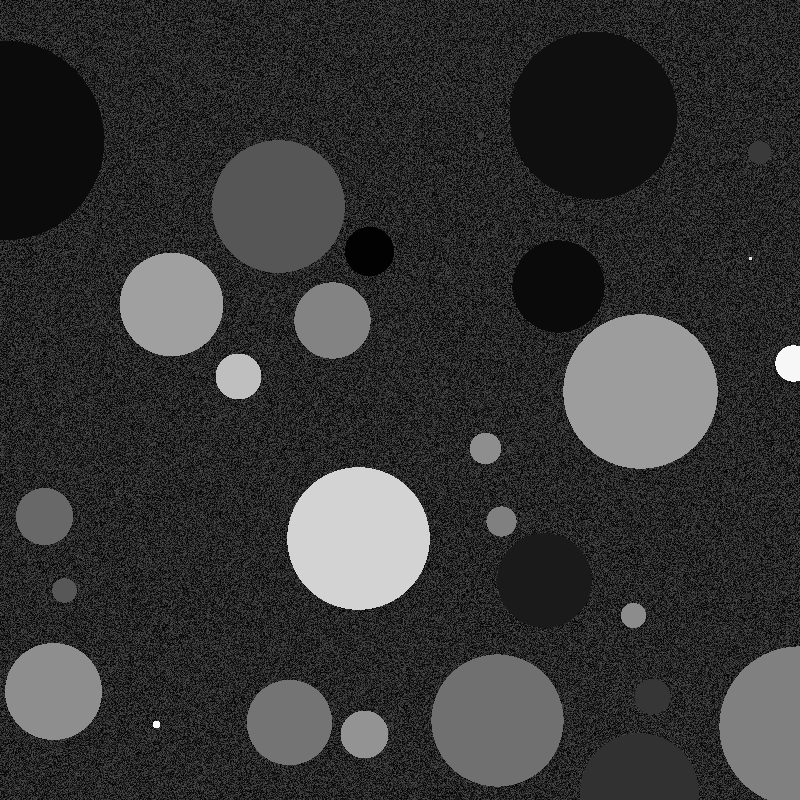
\includegraphics[width=\linewidth*3/4]{island_0024.png}
%  \caption{Island training image}
%  \label{fig:Islands}
%\end{figure}

\section{Topological Defect Tracking}

Previous work has been done demonstrating the viability of using basic neural networks to identify whether a given simulated data set contains a topological defect\cite{walters_machine_2019}. However, the paper was focused on simulated system states, consisting of molecule locations and orientations, rather than experimental image analysis. The utilized algorithm was purely for classification and did not give defect counts or locations. %Ask Adam how to discuss previous work
In order to make a system viable for usage with real experiments, we developed a pipeline that makes use of modern deep-learning object detection and image enhancement techniques capable of determining both the location and count of objects in an image. 

\subsection{Pipeline and Image Enhancement Motivation}
%ask adam about citing github projects
For object detection we used darkflow, a TensorFlow implementation of the YOLOv2 algorithm \cite{redmon_yolo9000:_2016} and offers improved performance when compared to the original YOLO algorithm\cite{redmon_you_2015}. YOLOv2 learns to perform both region proposal and region classification using the darknet-19 architecture. Training the region proposal mechanism is important for our task of object as detection algorithms that rely on traditional heuristic searches, such as R-CNN\cite{girshick_rich_2013} and its successors Fast R-CNN\cite{girshick_fast_2015} and Faster R-CNN\cite{ren_faster_2017}, would likely fail to identify defects as an object. Training and testing darkflow on a set of 100 simulated 200x200 images with each image containing 20 defects showed that this network is viable for detecting the locations of defects in simulation data. However, the usage of data enhancement techniques is necessary to make a network trained on simulated images viable for usage on real data. 

Machine learning algorithms, by nature, optimize themselves to perform as well as their architecture allows on the given training data. While this can lead to highly effective systems, it is the primary reason why training on a set of simulated data often makes the final model non-viable for usage in the real world; simulated data is highly predictable and clean while real-world data can have significant noise and variance in how key objects appear. By training on the simulated data, the system will over-fit\cite{lawrence_lessons_1997} \cite{lever_model_2016} on the very specific shapes, textures, and gradients produced by the simulation. %Since the objects of interest in the experimental data are almost guaranteed to not be as perfect as the ones in the simulation, the machine learning model will fail to identify them. 
Our solution for training a model on simulated data to analyze real data is to introduce various artifacts that mimic real-world inaccuracies into the simulated images.

\subsection{Standardization and Simulated Image Enhancement}

The first issue that needs to be dealt with is lighting and contrast. In simulated defect images, the intensity of a pixel ranges from perfectly black to perfectly white depending on the director orientation, maximizing the gradients and contrast in the image. The mean intensity of the image will also generally be around 0.5 on a scale from 0 (black) to 1 (white) since there is no offset to the image brightness. When using an experimental image, the difference in brightness between perfectly aligned and perfectly misaligned directors is much smaller than the full dynamic range of the image, causing smaller gradients. The average brightness of the experimental data is rarely 0.5, so what constitutes bright and dark pixels is more complex than just the intensity of the pixel. To make the simulation and experimental images as similar as possible in regards to average intensity and dynamic range, a variant of the basic feature standardization procedure\cite{aksoy_feature_2001} is used. Each pixel's intensity value is set according to the feature standardization formula

$$ x' = \frac{x - \Bar{x}}{6\sigma} +0.5 $$

where x' is the output pixel intensity, x is the input intensity of each pixel and $\sigma$ is the standard deviation of the global image pixel intensities. The output images have a mean pixel intensity of 0.5 and a dynamic range of six standard deviations. This procedure reasonably standardizes the lighting and contrast of the images regardless of the actual lighting and camera conditions, providing consistency for different data sets.

%In machine learning, training data is traditionally a hand labelled subset of the larger data-set to be analyzed. Training our algorithm with near-perfect auto-annotation simulation data, the model over-fits and fails to identify imperfect experimental objects. 
Adding imperfections to the simulated images emulates the experimental data and improve the robustness\cite{goodfellow_explaining_2014}\cite{bishop_training_1995} of the neural network model. Gaussian blurring, Fourier noise, randomized image variance, randomized lighting boundaries, and arbitrary objects target individually identified inconsistencies between simulation and experimental data. The alterations increase the image variety in our training data-set and teach the model that these imperfections are to be ignored when attempting to detect defects.

Due to the relatively low lighting of the experimental images, the camera read noise, generated by the camera hardware when reading information from the CCD, is significant relative to the signal size. Applying a 2-D discrete Fourier transform, the composition of the image is extracted in the frequency domain\cite{kaur_periodic_nodate} \ref{fig:Standardization and Noise}. The high frequencies, in the center of the image, contain the image information of interest, while the periodic read noise appears as regular lines. Removing the higher frequencies, the inverse Fourier transform yields the actual noise pattern of the camera. This characteristic camera noise is added as high-frequency noise to the simulated data set to increase similarity to experimental data.

\begin{figure}
  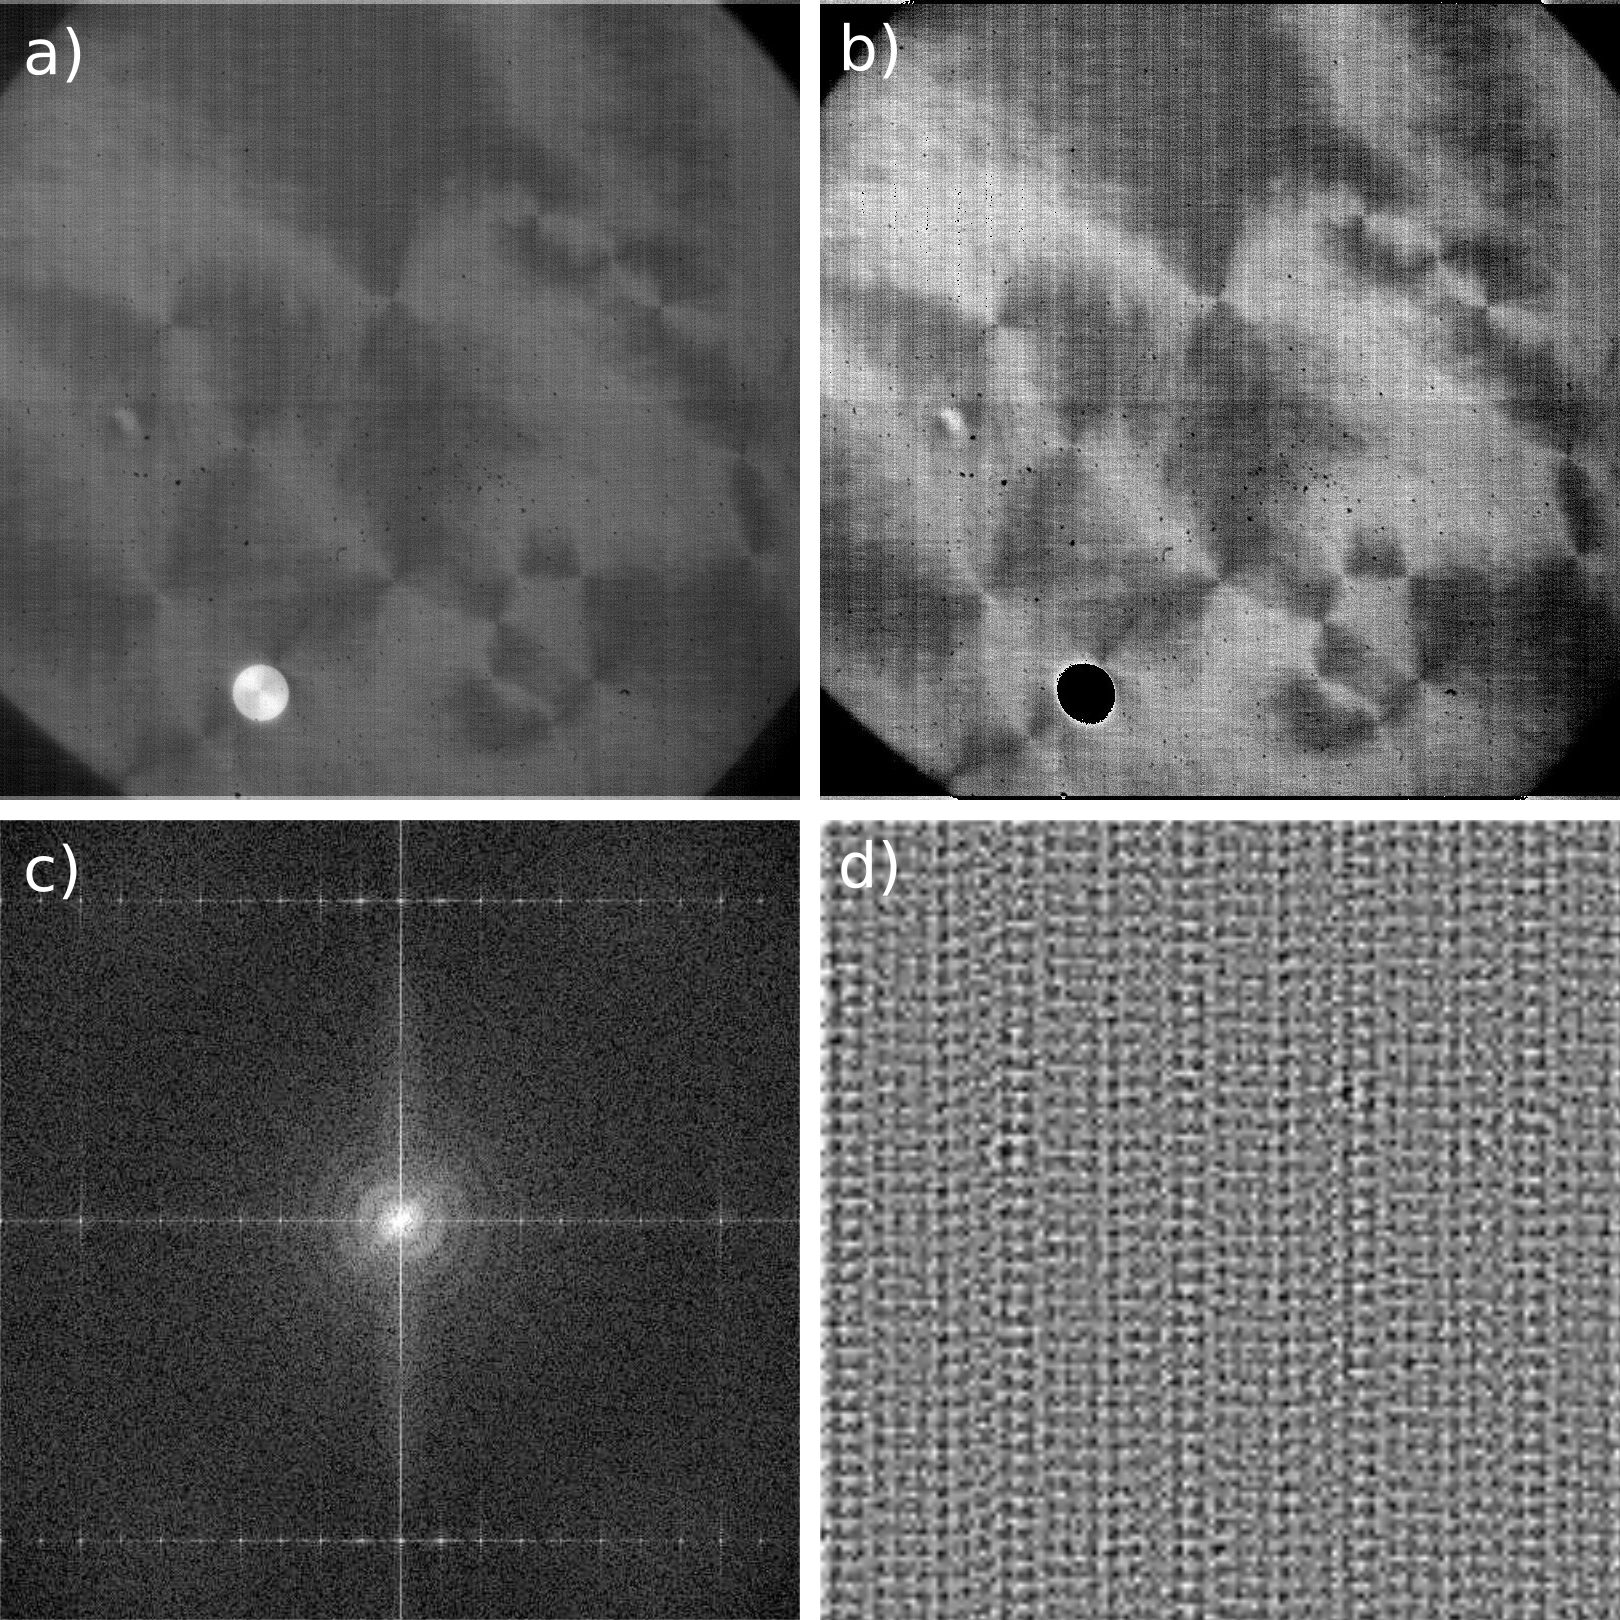
\includegraphics[width=\linewidth*3/4]{noiseExtraction.png}
  \caption{Image standardization and periodic noise extraction. A) Raw image with an island. B) Standardized image. C) Fourier transform of standardized image. D) Noise extracted from the image.}
  \label{fig:Standardization and Noise}
\end{figure}

Collecting experimental data, it is rare that perfect focus is consistently achieved. In the quenching experiment, there are additional film fluctuations as the pressure on the two sides of the film equalize causing a shifting focus point as the film moves. The lighting conditions can change significantly for different experimental setups. In particular, film thickness and camera settings have an impact on the intensities of light captured by the camera. Randomized Gaussian blurring emulates the non-perfect and variable focus of the experimental data. The overall brightness and dynamic range of the simulated images is randomized to prevent the model from being dependant on specific light intensities or gradient magnitudes unique to the simulation.

The final additions to the simulated images are randomized lighting domains and circular artifacts. Observing the pattern of defect detections from previous models, it was discovered that detections would be made along lines where the lighting abruptly shifts. The microscope aperture and the boundaries between CCD sectors, which consistently read slightly different pixel intensities, generate the light shifts. To prevent this, the simulation images were broken into four quadrants of randomized size, with each quadrant having slightly different brightness. False detections were also made around the boundaries of islands, which are regions in liquid crystal films with additional layers of material. Circles of random brightness were added to the simulation data to provide neutral examples \cite{koppel_importance_2006} of non-defect objects that should not be detected.

\subsection{Effects of Simulated Image Enhancements}

To evaluate the effectiveness of each component in the pipeline, several models were trained on simulated images enhanced by various combinations of pipeline components. The models were validated using a hand-annotated set of experimental images to determine how well they performed on real data relative to human performance.

In machine learning, there are multiple metrics used to determine how well a model performs. These metrics are designed to characterize the performance of the model in regards to the trade-off between the number and the accuracy of the detections reported. In our use case, we're interested in our model performing well in two aspects: precision, how many of our object detections are accurate, and recall, how many of the objects in the image we detect. Precision and Recall are defined as follows, where TP represents the true positive detections, FP represents the false positive detections, and FN represents the false negative detections.
$$ Precision = \frac{TP}{TP+FP} $$
$$ Recall = \frac{TP}{TP+FN} $$

The model provides a confidence score for each detection. A threshold is set to drop low confidence detections. A low threshold will increase recall while lowering precision; a high threshold will have the opposite effect by only using the few detections that have a high likelihood of being correct. mAP and peak F1 scores are used to characterize the model across all thresholds. AP is the Average Precision across all recall scores and is a general measure for the effectiveness of the model across all thresholds. mAP is the mean AP across all detected classes, however since we are only training to identify defects, mAP is effectively equivalent to AP. The F1 score is the harmonic mean of the precision and recall, and it provides an overall 'goodness' measure in regards to recall and precision at a specific threshold. We recorded the maximum F1 score of each model to provide a measure of the peak model performance when choosing an ideal threshold. The mAP\cite{everingham_pascal_2010} score can be thought of as measuring average performance without setting a minimum confidence threshold while peak F1\cite{chinchor_muc-4_1992} score measures the highest obtained performance over all thresholds. Using $p(r)$ to represent the precision at a given recall value and $n$ to represent the total number of detections, AP and F1 can be defined as follows:

\begin{figure}
  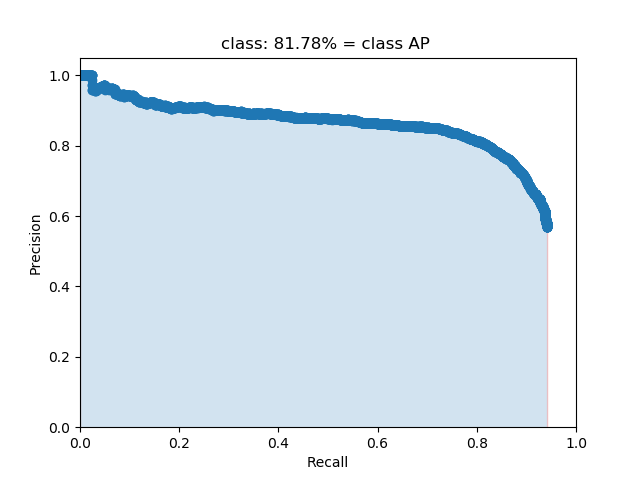
\includegraphics[width=\linewidth]{mAPCurve.png}
  \caption{Precision-Recall plot. mAP score is the percentage of area shaded between (0,0) and (1,1)}
  \label{fig:mAP score}
\end{figure}


$$ F1 = 2*\frac{Precision * Recall}{Precision + Recall} $$

$$ AP = \int_0^1 \!p(r) \, \mathrm{d}r $$
however, in order to use AP for real data the formula must be discretized into
$$AP = \sum_{r=1}^{n} p_{interp}(r)  $$
where
$$ p_{interp}(r) = max_{\bar{r}:\bar{r}>r} p(\bar{r})  $$
The usage of the max function smooths the AP curve, preventing the local dips at each false detection from affecting the global scoring.

Simulated training images enhanced with only blurring, random islands, random lighting quadrants, or randomized image brightness and contrast produced models that performed poorly on experimental images. On validation, these models received mAP scores of $<30\%$. Simulated images enhanced only with noise extracted using the Fourier transform produced a viable model, however the mAP score only reached $53.3\%$.

Adding multiple types of noise to the simulated images produced greatly improved models. Combining all types of artifacts produced a model with a mAP score of $59.0\%$, however this was outperformed by a model trained using only Fourier noise and randomized blurring which achieved a mAP score of $69.3\%$. Adding all forms of noise at a lower intensity to the simulated images produced a model with a mAP score of $74.9\%$. This suggests that a balance must be struck between making modifications and maintaining enough clarity to identify objects when training.

The original YOLOv2 \cite{redmon_yolo9000:_2016} paper reported an average mAP score of $73.4\%$ when tested using the Pascal VOC2012 test set, which puts the detection accuracy of our model trained with simulated images on par with models trained using real images. This supports the viability of training YOLO object detection models with simulated data for use on experimental data.

\subsection{Improvements Using the XY Model}
Models trained with data produced from the simulation using a Landau-Ginzberg implementation of the XY model yielded accuracy improvements for the final models. Landau-Ginzberg simulations provide thermal noise, as we see in our real data, and emulate natural defect systems. With no image modifications, a model trained on simulated images from the XY simulation attained a $47.4\%$ mAP score, a significant improvement over the 2\% achieved with the model trained on the raw random defects data. 
%TODO:
%   - We should reference the performance of the raw Random Defect simulation
\begin{figure}
  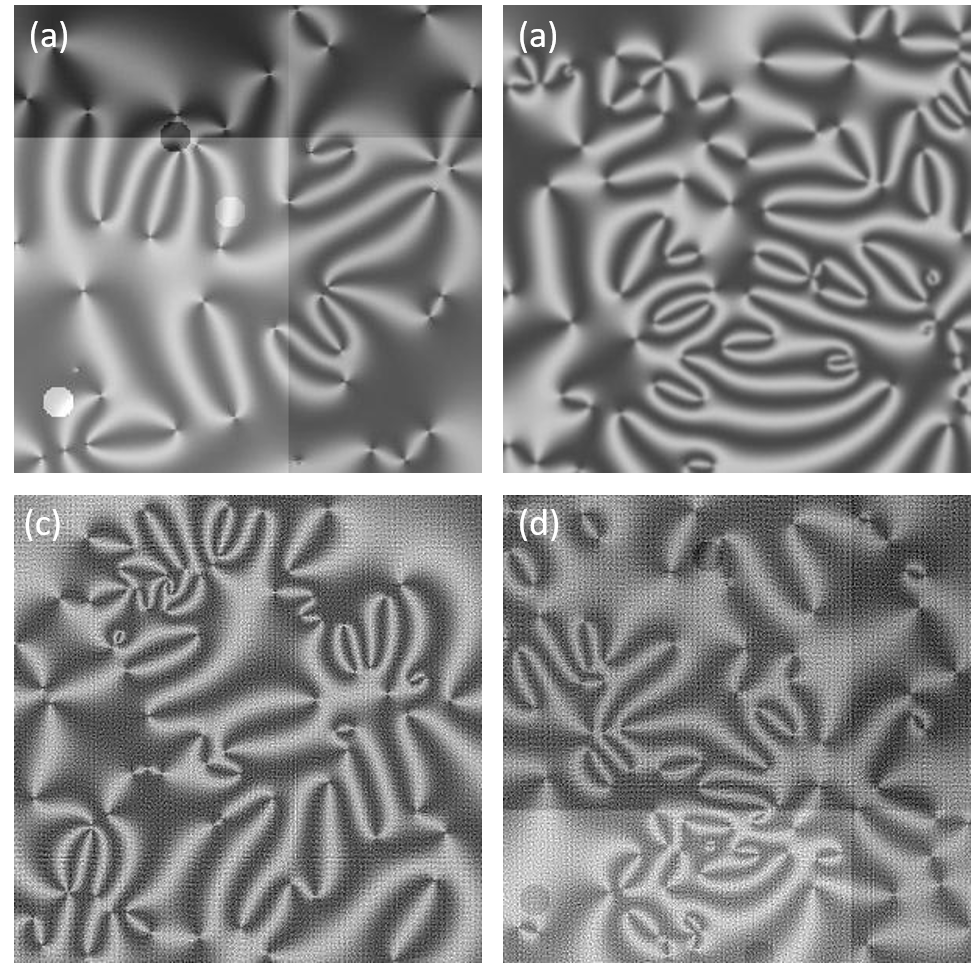
\includegraphics[width=\linewidth*3/4]{imageEnhance.png}
  \caption{Simulated images enhanced with various types of noise. (a) Image with dramatic lighting shifts and added circles (islands) (b) Image with Gaussian blurring (c) Image with Fourier noise (d) Image with all three}
  \label{fig:Image Enhancement}
\end{figure}

\begin{table}[]
\resizebox{\columnwidth}{!}{%
\begin{tabular}{lll}
\hline
\multicolumn{3}{l}{Table 1}                                                                                                                   \\
\multicolumn{3}{l}{\textit{\begin{tabular}[c]{@{}l@{}}Scoring of Models Trained\\   on Simulated Images with Various Artifacts\end{tabular}}} \\ \hline
{\ul Artifacts Added}                               & {\ul Peak F1}                      & {\ul mAP}                                    \\
LG, L-FN, L-RV, L-RB, L-GB, L-DC, RD, LR            & 0.811                                    & 0.818                                        \\
LG, L-FN, L-RV, L-RB, L-GB, L-DC, RD                & 0.817                                    & 0.808                                        \\
LG, FN, RV, RB, GB, DC, RD                          & 0.806                                    & 0.783                                        \\
L-FN, L-RV, L-RB, L-GB, L-DC, RD                    & 0.754                                    & 0.749                                        \\
FN, RB                                              & 0.744                                    & 0.738                                        \\
FN, RV                                              & 0.726                                    & 0.725                                        \\
FN, RV, RB, GB, DC, LT                              & 0.740                                    & 0.700                                        \\
FN, GB                                              & 0.707                                    & 0.693                                        \\
FN, RV, RB, GB, DC, RD                              & 0.683                                    & 0.663                                        \\
FN, RV, H-RB, GB, DC, RD                            & 0.661                                    & 0.643                                        \\
FN, RV, RB, H-GB, DC, RD                            & 0.635                                    & 0.626                                        \\
FN, RV, RB, GB, H-DC, RD                            & 0.632                                    & 0.620                                        \\
H-FN, RV, RB, GB, DC, RD                            & 0.640                                    & 0.617                                        \\
FN, RV, RB, GB, DC                                  & 0.613                                    & 0.590                                        \\
FN, H-RV, RB, GB, DC, RD                            & 0.587                                    & 0.579                                        \\
FN                                                  & 0.569                                    & 0.533
                                     \\
LG                                                  & 0.513                                    & 0.474 
\\
RB                                                  & 0.442                                    & 0.270                                        \\
RV                                                  & 0.423                                    & 0.260                                        \\
GB                                                  & 0.296                                    & 0.116

\\ \hline
                          
\end{tabular}%
}

\resizebox{\columnwidth}{!}{%
\begin{tabular}{lll}
\multicolumn{3}{l}{\textit{Key}}                                                            \\
FN: Fourier Noise       & GB: Random Gaussian Blurring  & LT: Longer Training Time          \\
RV: Random Variance     & DC: Randomized Decross Angle  & L-XX: Lowered randomization of XX \\
RB: Random Boundaries   & RD: Randomized Defect Number  & H-XX: Higher randomization of XX  \\
LR: Long Simulation Run & LG: Used LandauGin Simulation &                                  
\end{tabular}%
}
\end{table}

The Landau-Ginzberg simulations are highly time-dependent with defect counts following a power function. This means that a linear reduction in defect number requires an exponential amount of time. If we train a model with only early time simulation images, where there is a high density of defects in the training data, the model will perform worse on images with a lower defect density. As such, the best performing models require long simulation runs to generate training data with a wide variety of defect densities. 

Similar to the random defect simulation data, the best results are attained with a lower intensity of many different forms of noise, achieving a mAP score of $81.8\%$. A full accounting of the artifacts added when training models and the evaluation metrics for each model can be found in Table 1.

\subsection{Model Applications}

When applying the model to data, a threshold needs to be set to eliminate low-confidence detections. To maximize the trade-off between precision and recall, the threshold corresponding to the model's peak F1 score is used. To evaluate the applied performance of the system, we use the top-scoring model which employed Landau-Ginzberg simulation and moderate levels of image enhancement.% with a specified threshold of 0.481.  

A straightforward applications of the model is counting the defects per frame in a video. The model results, as seen in  in Figure \ref{fig:HumanVMachine} a, c, and e, show a high similarity to the counts made by a human.
The average nearest neighbour calculation, a value of interest to those studying topological defect behaviour in films, is a more involved calculation requiring defect locations to compute the distance to the closest neighboring defect. \ref{fig:HumanVMachine}b, d, and f show a result similar to that calculated from human annotated defects. %ADAM, Add the reason why this is significant for physics please?

\begin{figure}
  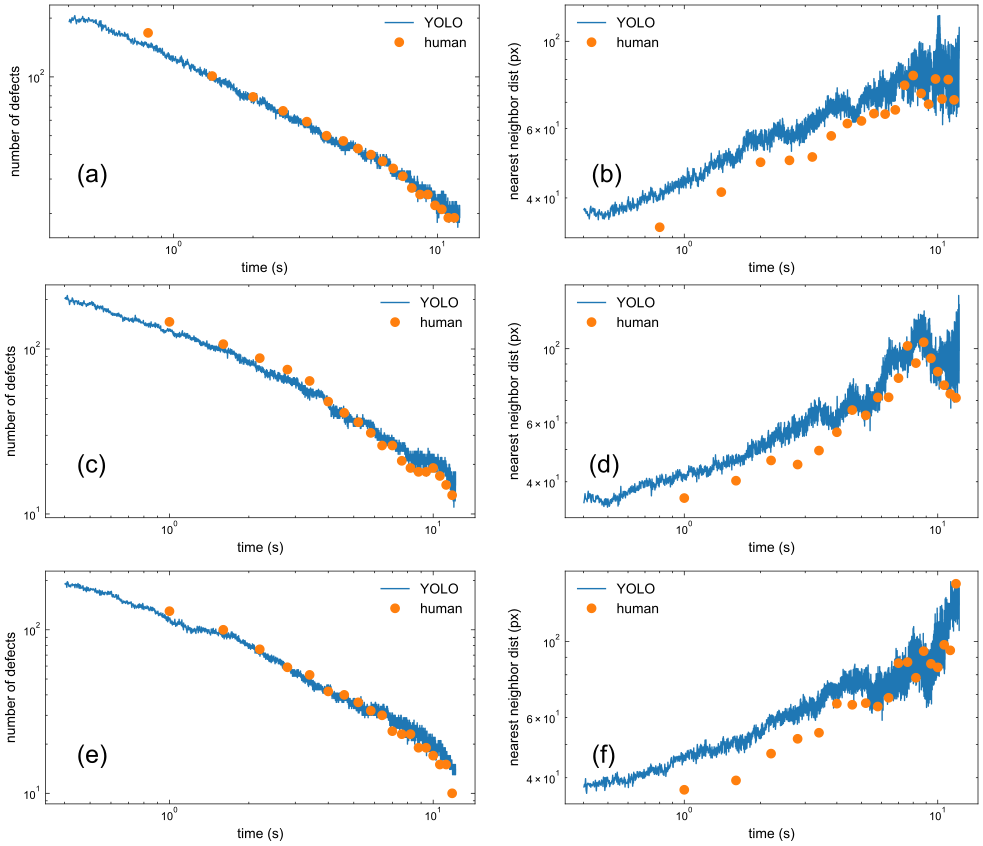
\includegraphics[width=\linewidth]{humanVmachineAllR.png}
  \caption{a,c,e) show Number of Defects vs. Time for 3 separate videos. b,d,f) show Nearest Neighbour vs. Time for 3 different videos.}
  \label{fig:HumanVMachine}
\end{figure}

Reliable defect tracking requires the model to be consistently capable of precisely locating defects over a larger number of frames -- a common yet challenging goal in the machine learning paradigm. We make use of the Trackpy Python module, a package of functions specializing in particle tracking, to link identified objects through consecutive images over time. The end result is a linked path for each defect, as seen in Figure \ref{fig:tracks}.

\begin{figure}
  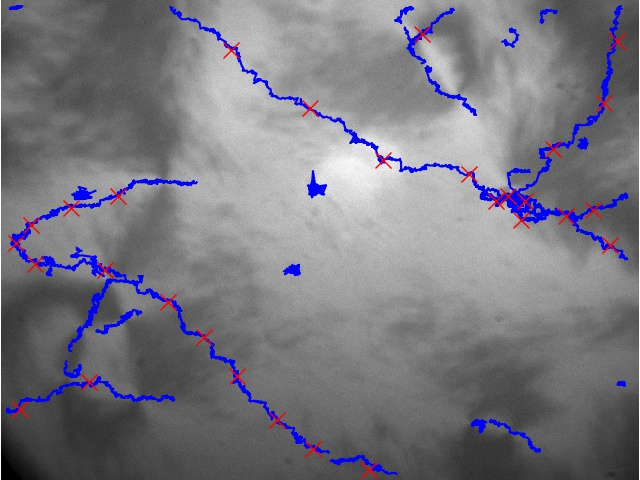
\includegraphics[width=\linewidth]{track.jpg}
  \caption{Computer tracked paths represented by blue lines. Human annotations represented by red Xs.}
  \label{fig:tracks}
\end{figure}

To numerically rate the performance of our defect tracking, we compare the track to human annotated defect locations. Error is calculated by taking the root mean square of the distance in pixels between each human annotated defect location and the nearest neighbour path. For the test case in \ref{fig:tracks}, using the best performing model, we found this value to be 1.03 pixels. This shows that our machine learning pipeline is capable of tracking objects to a similar quality as a human, making it a viable method for high precision automation.

\subsection{Computational Performance}

Running the model on 1104x800 images, it takes approximately 0.07 seconds per image with an 8 second startup overhead on a 2017 GeForce$^{\tiny{\textregistered}}$ GTX 1080 GPU. When tested on an i7-7700K CPU, the model took 4.62 seconds per image with a 10 second startup overhead. When training on the aforementioned GPU, it took 0.51 seconds per iteration using a batch size of 8 with a 12 second startup overhead, or approximately 0.064 seconds per image. When training on the CPU, the time per image was approximately 3 seconds.   % On my laptop each image takes about 1-2 seconds (I did 5k images in about 1 hour 45 minutes) on i7-4720HQ @ 2.60GHzx4. This may be because I was running off solid state memory perhaps? Because my CPU is almost definitely slower than a 7700k. Other possibility is system state, perhaps from not restartign for a while, or using another program? Honestly not sure.
This demonstrates the viability of using the system for rapid image data analysis, especially when used in conjunction with a modern GPU. Using a GPU, a model trained for 40 epochs on a training-set of 1000 images takes approximately 1-1.2 hours.
Training an identical model on the CPU is estimated to take between 20-40 hours, however this was not explicitly measured.

\section{Results and Discussion}
\blindtext{}


% SPECIFICS TO BE COMPLETED WITH/BY ADAM
%Abstract
%Expanded Explanation of XY model and simulations in Introduction/Experimental setup
%Citations for topological defects and XY model
%Results and Discussion
%Github citation and material citation (idea how to cite Kirsten's dissertation)
%Potentially motivation for nearest neighbor/defect counts in Applications of model
%Proper way to reference a figure
%Overall review of paper for compliance with literary standards







%\begin{figure}[H]
%\centering
%\includegraphics[keepaspectratio=true,width=\columnwidth]{fig1-jem.png}
%\caption{write figure caption here}
%\label{fig:labelfighere}
%\end{figure}
%
%\bibliographystyle{apsrev4-1}
%\bibliography{../bibfilenamewithout.bib} % this is .bib file
\bibliographystyle{apsrev4-1}
\bibliography{MLFilms.bib,references.bib}

\end{document}